\subsection{Examples}

\begin{concept}{Interrupt Basics}\\
Key concepts for interrupt handling:
\begin{itemize}
  \item \textbf{Interrupt Sources}:
    \begin{itemize}
      \item Hardware interrupts from peripherals
      \item Software interrupts (SVC)
      \item System exceptions
    \end{itemize}
  \item \textbf{Configuration Steps}:
    \begin{itemize}
      \item Enable specific interrupt source
      \item Install interrupt handler
      \item Configure interrupt priority
      \item Enable global interrupts
    \end{itemize}
  \item \textbf{Handler Requirements}:
    \begin{itemize}
      \item Predefined names from vector table
      \item No return values allowed
      \item Must clear interrupt flags
      \item Save/restore used registers
    \end{itemize}
\end{itemize}
\end{concept}

\begin{example2}{Timer Interrupt Configuration}\\
Configuring Timer 2 interrupt:

1. Handler definition:
\begin{lstlisting}[language=armasm, style=basesmol]
    AREA    handlers, CODE, READONLY
    
    EXPORT  TIM2_IRQHandler
TIM2_IRQHandler
    PUSH    {R4-R6}          ; Save registers
    ; Handle interrupt
    POP     {R4-R6}          ; Restore registers
    BX      LR               ; Return
\end{lstlisting}

2. Enable interrupt (IRQ28):
\begin{lstlisting}[language=armasm, style=basesmol]
    AREA    startup, CODE, READONLY
    
SETENA0     EQU     0xE000E100  ; Interrupt enable register
    
    ; Enable Timer 2 interrupt
    LDR     R7, =SETENA0
    MOVS    R6, #1           ; Set bit
    LSLS    R6, #28          ; Shift to IRQ28
    STR     R6, [R7]         ; Enable interrupt
\end{lstlisting}
\end{example2}

\begin{example2}{Data Consistency Protection}\\
Protecting shared data access:

\begin{lstlisting}[language=C, style=basesmol]
// Global time counters accessed by ISR
volatile uint32_t minutes = 0;
volatile uint32_t hours = 0;

// Timer ISR updates counters
void TIM2_IRQHandler(void) {
    minutes++;
    if (minutes >= 60) {
        minutes = 0;
        hours++;
    }
    // Clear interrupt flag
}

// Main code reading counters
void read_time(uint32_t *min, uint32_t *hr) {
    // Disable interrupts to read consistent values
    __disable_irq();
    *min = minutes;
    *hr = hours;
    __enable_irq();
}
\end{lstlisting}

Assembly equivalent:
\begin{lstlisting}[language=armasm, style=basesmol]
read_time
    PUSH    {R4-R5, LR}
    CPSID   i               ; Disable interrupts
    
    LDR     R4, =minutes    ; Load minutes
    LDR     R2, [R4]
    STR     R2, [R0]        ; Store to output
    
    LDR     R5, =hours      ; Load hours
    LDR     R3, [R5]
    STR     R3, [R1]        ; Store to output
    
    CPSIE   i               ; Enable interrupts
    POP     {R4-R5, PC}
\end{lstlisting}
\end{example2}

\begin{KR}{Interrupt Handler Implementation}\\
Guidelines for implementing interrupt handlers:

1. Handler structure:
\begin{lstlisting}[language=armasm, style=basesmol]
handler_name
    PUSH    {R4-R6}          ; Save used registers
    
    ; Check interrupt flags
    ; Handle interrupt condition
    ; Clear interrupt flags
    
    POP     {R4-R6}          ; Restore registers
    BX      LR               ; Return from handler
\end{lstlisting}

2. Register preservation:
\begin{itemize}
  \item R0-R3: Automatically saved by hardware
  \item R4-R11: Must be preserved if used
  \item R12: Can be used freely
  \item LR: Contains special EXC\_RETURN value
\end{itemize}

3. Critical section handling:
\begin{lstlisting}[language=armasm, style=basesmol]
    ; Disable all interrupts
    CPSID   i
    
    ; Critical section code
    ; Access shared resources
    
    ; Enable interrupts
    CPSIE   i
\end{lstlisting}
\end{KR}

\begin{example2}{NVIC Configuration}\\
Complete interrupt system setup:

\begin{lstlisting}[language=C, style=basesmol]
void init_timer_interrupt(void) {
    // Configure timer peripheral
    TIM2->PSC = 7199;        // Prescaler
    TIM2->ARR = 9999;        // Auto-reload value
    TIM2->DIER |= 1;         // Enable interrupt
    TIM2->CR1 |= 1;          // Enable timer
    
    // Configure NVIC
    NVIC_SetPriority(TIM2_IRQn, 2);  // Set priority
    NVIC_EnableIRQ(TIM2_IRQn);       // Enable IRQ
    
    __enable_irq();          // Enable global interrupts
}

// Timer 2 interrupt handler
void TIM2_IRQHandler(void) {
    if (TIM2->SR & 1) {      // Check update flag
        // Handle interrupt
        TIM2->SR &= ~1;      // Clear flag
    }
}
\end{lstlisting}

Assembly equivalent:
\begin{lstlisting}[language=armasm, style=basesmol]
TIM2_BASE    EQU     0x40000000
TIM_SR       EQU     0x10
TIM_DIER     EQU     0x0C
SETENA0      EQU     0xE000E100

    ; Enable timer interrupt
    LDR     R0, =TIM2_BASE
    LDR     R1, [R0, #TIM_DIER]
    ORRS    R1, #1
    STR     R1, [R0, #TIM_DIER]
    
    ; Enable in NVIC
    LDR     R0, =SETENA0
    MOVS    R1, #1
    LSLS    R1, #28         ; IRQ28
    STR     R1, [R0]
\end{lstlisting}
\end{example2}

\begin{remark}
Important considerations:
\begin{itemize}
  \item Always clear interrupt flags
  \item Minimize time in interrupt handlers
  \item Protect shared data access
  \item Consider interrupt priorities
  \item Avoid deadlocks with nested interrupts
\end{itemize}
\end{remark}

\section*{CT1 Übungsaufgaben}
\section*{Exceptional Control Flow}
\section*{Aufgabe 1}
Um eine Interrupt Quelle nutzen zu können muss der entsprechende Interrupt enabled werden (neben anderen Konfigurationsaktionen).

Annahme: Sie müssen für den Timer 2 einen Handler installieren und den Interrupt enablen.

\begin{enumerate}
  \item Wie heisst der Interrupt Handler für Timer 2?
\end{enumerate}

Öffnen Sie dazu in irgendeinem der Praktika Projekte das File startup\_ctboard.s und suchen sie nach dem passenden Handler Namen in der $\qquad$ Vectors Tabelle.\\
Tipp: Suchen Sie nach TIM2...\\
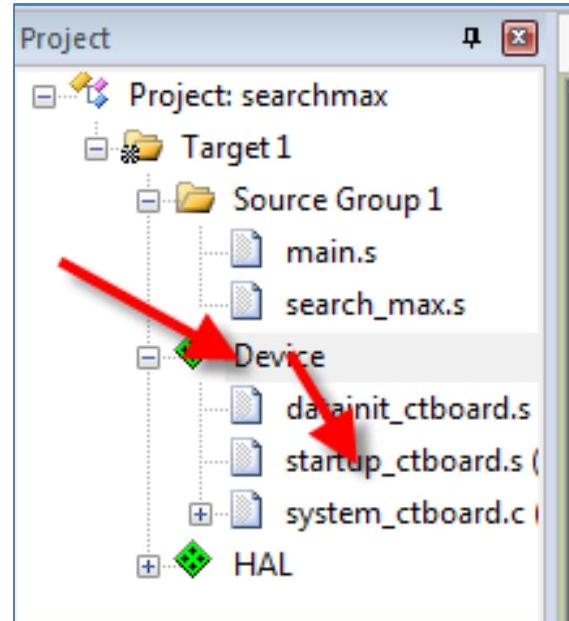
\includegraphics[width=\linewidth]{images/2025_01_02_1e89fec346403e1ae751g-1}

\section*{TIM2\_IRQHandler}
\begin{enumerate}
  \setcounter{enumi}{1}
  \item Welche Interrupt Nummer hat dieser externe Interrupt? Zählen Sie vom ersten externen Interrupt, beginnend mit 0, bis zum entsprechenden Interrupt Handler.
\end{enumerate}

28\\
3) Geben Sie die Assembler Instruktionen an um diesen Interrupt mit der gegebenen Interrupt Nummer zu enablen - siehe Vorlesung Seite 27: „Interrupt Enable Registers".

\begin{verbatim}
SETENAO EQU OxEOOOE100
    LDR R7,=SETENAO
    MOVS R6,#1
    LSLS R6,#28
    STR R6,[R7]
\end{verbatim}

\section*{Aufgabe 2}
Enabling von Interrupt Quellen, wie in Aufgabe 1 behandelt, dient zur initialen Konfiguration von Interrupts. Im Betrieb ist es aber unter Umständen nötig alle Interrupts kurzfristig auszuschalten und danach wieder einzuschalten.

\begin{enumerate}
  \item Was kann ein Grund sein für ein solches kurzfristiges Aus- und wieder Einschalten?
\end{enumerate}

Data Konsistenz: z.B. eine Interrupt Service Routine eines Timers unterhält zwei Zähler,\\
einen für Minuten und einen für Stunden. Beim Übergang von Minute 59 zu 0 wird der

Stundenzähler um eins erhöht. Eine andere Routine welche diese beiden Zähler ausliest\\
muss dafür sorgen dass kein Interrupt passiert zwischen dem Zugriff auf diese beiden Zähler.\\
2) Wie schalten Sie alle Interrupts in Assembler aus? Wie ein?

Ausschalten:


\textbf{CPSID i}


Einschalten:\\
CPSIE i\\
3) Wie schalten Sie alle Interrupts in C aus? Wie ein?

Ausschalten:

\begin{verbatim}
_disable_irq();
\end{verbatim}

Einschalten:

\begin{verbatim}
    __enable_irq();
\end{verbatim}

\section*{Aufgabe 3}
Der ARM Prozessor rettet beim Abarbeiten eines Interrupts gewisse Register auf den Stack bevor die ISR (Interrupt Service Routine) ausgeführt wird - und restauriert diese nach Beendigung der ISR automatisch.

\begin{enumerate}
  \item Wenn Sie in Ihrer ISR die Register R0-R6 verwenden, welche dieser Register müssen Sie auf den Stack pushen weil sie nicht schon automatisch vorher gerettet wurden?
\end{enumerate}

\begin{verbatim}
PUSH {R4-R6} ; R0-R3 wurden schon automatisch gerettet
\end{verbatim}

\begin{enumerate}
  \setcounter{enumi}{1}
  \item Wie Unterscheidet sich in der Programmierung eine ISR von einer „normalen" Funktion?
\end{enumerate}

Jede ISR hat einen vordefinierten Namen (von der $\qquad$ Vectors Tabelle vorgegeben).

Eine ISR kann keine Werte zurückgeben (ist in C eine void iss\_name (void) Funktion).

Eine ISR muss gegebenenfalls den Interrupt zurücksetzen so dass er nicht permanent feuert.